\documentclass{template}

\usepackage{etoolbox}
\usepackage{epstopdf}


\begin{document}
\newcommand\MyHead[2]{%
	\multicolumn{1}{| c |}{\parbox{#1}{\centering #2}}
}

\makeatletter
\patchcmd{\maketitle}{\@copyrightspace}{}{}{}
\setlength{\@fptop}{5pt}
\makeatother

	\title{Mining Utility Functions Based on User Ratings}
	\author{COMP5331 Project Report\\Sepanta Zeighami\\20213665}
    \maketitle

\begin{sloppy}
	\begin{abstract}
		We propose a method to use ratings provided by users on database items to understand users' overall preferences. The amount of user rating data available, on for instance e-commerce platforms, enables us to discern each user's preferences, such as whether the user prefers better quality over lower price or not. Thus, we can examine how much value each user attaches to different attributes of the items. By inferring such information from each user's ratings, we aim at understanding how the users in general perceive and evaluate different features of the items in the database. To this end, we propose different methods to build the probability distribution of the users' preferences based on the ratings they provide on different items in a database. We suggest to model the preferences of the users using linear utility functions. We further use Gaussian mixture models and kernel density estimation techniques to build the probability distribution of the preferences. This allows us to answer questions such as what is the probability of a user paying more attention to one attribute of an item compared to another. Having access to such an information is useful for businesses as well as research fields that deal with utility functions and user preferences.
	\end{abstract}
	
	\section{Introduction}
	By the proliferation of the amount of data available on the internet, opinions expressed by users, either explicitly or implicitly, can be found on various parts of the web. As an example, many websites allow users to provide feedback, reviews and ratings regarding the items they have purchased or used. Thus, a possible use of the data is to deduce how different users perceive various items on which the opinion of some of the users is known. 
	
	As an example, consider a hotel booking website. Users of the website might be able provide reviews and ratings on the hotels they have booked. Furthermore, a database of hotels will exist that contains different information about different hotels. Based on these together, it is possible to infer how different features of the hotels affect the way consumers evaluate them.
	
	To be more specific, assume that in the database of the hotels, the information available about each hotel contains its price, distance from downtown and size of the rooms. A problem of interest, then, is that when users are booking a hotel, how much value do they attach to each attribute of the hotels. Note that there is a trade-off between different qualities of the hotel. For example, a hotel with a better price is usually in a worse location. Furthermore, the users have different preferences and criteria in mind in their decision making. A rich businessman, for instance, might care less about the price of a hotel compared with a student.
	
	As mentioned, it might be of interest, for the hotel website owner for instance, to know how different users perceive different hotels. This information can be used for different purposes. One of the applications can be suggesting hotels to the users in recommendation systems. Additionally, the owner can use this information for policy making. For example if the majority of the users care much more about the price of the rooms, it might make sense for the website to contain a larger number of low-priced hotels and fewer expensive ones.
	
	To be able to answer such questions, we need to be know what the probability of a specific user having a specific set of preferences is. In more mathematical terms, we need to have access to the probability distribution of the user's preferences. To denote the user's preferences, we use utility functions, which, informally, are functions that quantify the satisfaction a user gets from a specific point. Using this concept, the problem translates into finding the probability distribution of the utility functions of users. 
	
	Knowing the probability distribution of utility functions can help businesses make more informed decisions, as mentioned above. Furthermore, utility functions, recently, have been used in various research fields (such as \cite{utilUse1, utilUse2}). Knowing the distribution of utility functions can help enhancing the results in those fields as it can provide more realistic information.
	
	However, work in this area have been mainly limited to understanding a specific user's preferences. Different methods have been proposed to predict user's choices given information on the user or his or her previous choices and information about the other user's preferences. However, the literature has come short in analyzing the existent information on current users instead of predicting the future.
	
	\subsection{Contributions}
	Motivated by this, in this project, we aim at developing a method in order to infer the probability distribution of the \textit{utility functions} of the users of a database, given a set of ratings on a number of the items in the database provided by a set of the users. In the hotel booking example, the mentioned ratings can be the rating a user provides on a hotel. We build the probability distribution to be able to answer the question such as what is the probability of a user attaching more value to price compared to location of the hotel.
	
	In solving this problem, our major contributions can be summarized as follow.
	\begin{itemize}
		\item{We propose the use of linear utility functions to model user preferences.}
		\item{We estimate the probability distribution of utility functions using Gaussian mixture models and kernel density estimation.}
		\item{We conduct empirical studies to evaluate our proposed methods.}
	\end{itemize}
	
	\textbf{Organization.} We first give a summary on the relevant works in the literature in section 2. Then, we provide the definition of the problem addressed in this paper as well as the assumptions behind our model in section 3.In section 4, we explain how we find a specific user's utility function. After that, we provide our methods to build a probability distribution of utility functions in section 5. We present our experiments in section 6 and conclude the paper in section 7.
	
	
	
	
	
	

\section{Related Works}
	Mining utility functions and discovering user preferences users has been explored in the literature before. Recommender systems, machine learning approaches in preference learning as well as preference elicitation are research fields that are closely related to our work.
	
	\textbf{Recommender systems}. Recommender systems \cite{Recommender:Rashid, Recommender:Burke} aim at predicting a new user's preferences based on the information about the previous users. Two general approaches is to either group the users together based on their similarities or to utilize the similarity in the contents of the items. Although approaches similar to recommender systems can be taken when inferring the distribution of the utility functions, the problem addressed in this project differs from the recommender systems in that it does not involve predicting a new user's preferences based on the information available about the new user. 
	
	\textbf{Preference learning}. Machine learning approaches \cite{GP:Chu, GP:Houlsby} have been developed to learn the and predict the preferences of a specific user. These approaches try to learn the utility function of a specific user based on the preferences expressed by the user and based on that, predict user's preferences on unseen items. These methods mainly focus on predicting user's preferences based on some previous knowledge. Although, in our approach, we can use models proposed in this area to learn a specific user's preferences, our focus is on understanding the distribution of the preferences of the users rather than predicting the preferences of the users on unseen data.

	\textbf{Preference elicitation}. Another area related to this topic is preference elicitation \cite{PE:Blum} in which queries are asked from the user to understand their preferences. This area, closer to preference learning, differs from our project in that we aim at understanding the user preferences from the ratings available and not asking questions from the users.

	The work in this project differs from the previously existing works in that, we analyze the provided ratings in the context of the items in the database. As such, our work is addressing a different problem compared to the vast majority of the literature that focuses on prediction of user preferences and recommendation of items to the customers based on the preferences.

\section{Definitions and Assumptions}
Before being able to address the problem introduced above, we first need to give a formal definition of the problem. Here, we formalize the notation used in the rest of this paper and give a more rigorous definition of the concepts and the problem addressed in this paper.

\subsection{Utility Functions}
The ultimate aim of this project is to gain more insight in to the decision making process of the users of a set of items available in a database. To understand the users better, we need to be able discern how they evaluate different choices (i.e. the items in the database) they have. For this, we introduce the concept of \textit{utility functions}. Utility functions are used to quantify the ``satisfaction'' or ``happiness'' a user derives from a specific point from a database.

\medskip
\indent \textit{Definition 1.}  \textbf{Utility function.} On a database $D$, a \textit{utility function} $f$ is a mapping $f: D \rightarrow \mathbb{R}$. For a point $p$, $p \in D$, $f(p)$ denotes the \textit{utility} of a user with the utility function $f$ derived from the point $p$.
\medskip

\begin{table}
\centering
\begin{tabular}{|c | c | c | c |} \hline
name &	price & \MyHead{2.3cm}{distance from downtown} & size \\\hline
  Holiday Inn            &0.94	    & 0.18	    & 0.28  \\\hline
  Shangri la 	          &0.91 	    & 0.39	    & 0.13  \\\hline
  Intercontinental    &0.62      & 0.24   	    & 0.74  \\\hline
  Hilton             	&0.15        &0.77	    & 0.61  \\\hline
\end{tabular}
\caption{Hotels in the database. The higher the value, the more favourable the criterion is (including price)}
\label{table:1}
\end{table}
\begin{table}
\centering\begin{tabular}{|c | c | c | c |} \hline
name &	price & \MyHead{2.3cm}{distance from downtown} & size \\ \hline
  Alex   &	0.8    & 0.05	    & 0.15  \\\hline
  Jerry   &	0.75    & 0.2	    & 0.05 \\\hline
  Tom   &	0.4    & 0.1	    & 0.5  \\\hline
  Sam   &	0.05    & 0.55   & 0.4  \\\hline
\end{tabular}
\caption{Utility functions of the users}
\label{table:2}
\end{table}
\begin{table}[t]
	\centering\begin{tabular}{|c | c | c |} \hline
		User  &	Hotel & Rating \\ \hline
		Alex  &	Hilton& 0.25  \\\hline
		Alex  &	Shangri la & 0.75  \\\hline
		Tom &	Shangri la  & 0.45 \\\hline
		Jerry   &	Holiday Inn   & 0.75  \\\hline
		Sam   &	Intercontinental    & 0.45  \\\hline
	\end{tabular}
\caption{Ratings provided by the users}
\label{table:3}
\end{table}
A utility function provides us with a means to measure a user's satisfaction. Each user has a specific utility function. In other words, we can define a user by his or her utility function. Thus, the notions of ``utility function" and ``user" are used interchangeably in this paper. As an example, on the database shown in Table 1, a user can have the utility function $f(price, distance, size)$ = 0.8 $\times$ price + 0.05 $\times$ distance + 0.1 $\times$ size. This means that this user attaches more value to the price of the hotel in comparison with the distance or the size. Based on this function we can calculate the utility of the user from different points. For instance, the utility of the user from Hilton Hotel is $f(0.15, 0.77, 0.61) = 0.8 \times 0.15 + 0.05 \times 0.77 + 0.15 \times 0.61$ = $0.25$. A user is more satisfied if the value of his or her utility function is higher. 

Note that the utility function of a user is defined on the domain of the database. That is, if the database the utility function is defined on is a database consisting of $n$ points, then input to the the utility function of a user can only be one of the $n$ points in the database. As a result, we can represent the utility function of a user with an $n$-dimensional vector whose $i$-th element is the utility the user derives from the $i$-th point in the database. In other words, if $p_i$ is the $i$-th point in the database $D$, and $f_i$ is the utility the user derives from $p_i$ (in the previous notation $f(p_i) = f_i$), then we can write
\[f = \left( \begin{array}{c}
f_1 \\
f_2 \\
\vdots\\
f_n \end{array} \right)\].

A class of utility functions that will be used in the rest of this paper is the class of \textit{linear utility functions}. A linear utility function is a function that can be written as the linear combination of the attributes of its input.  

\medskip
\indent \textit{Definition 2.}  \textbf{Linear Utility functions.} On a $d$-dimensional database $D$, a utility function $f$ is a \textit{linear utility function} if there exists a single $d$-dimensional vector $w$ for all the points $p, p \in D$, for which $f(p) = \sum_{i = 1}^{d} w_i \times p_i$, where $w_i$ is the $i$-th element of $w$ and $p_i$ is the value of the $i$-th dimension of the point $p$. Alternatively, we can write $f(p) = p\cdot w$. We call $w_i$ the weight the user attaches to the $i_th$ dimension. We can denote the utility function $f$ by its weight vector $w$.
\medskip

In the example above, the utility function of Alex was a linear utility function as it was defined as the linear combination of the three dimensions of the database. Obviously, not all the utility functions are linear, and such1 weight vector might not exist.

In general, we do not know the utility function of the users. we try to learn about it based on users' behavior or the information they provide. One of the ways we can obtain such an information is through users' feedback. For example, many websites allow their customers to rate and evaluate the items they buy. Such user ratings are a way customers express how satisfied they are with an item. More specifically, the ratings are a quantification of the satisfaction of the users, or in the terms defined above, the utility a user derives from an item. Therefore, we can define a rating as follows.

\medskip
\indent \textit{Definition 3.}  \textbf{Ratings.} On a database $D$, for a user with utility function $f$ a rating is an observed value of the utility function of the user. That is if the user provides a rating $r$ on an item $p$ from the database, then $f(p) = r$.
\medskip

Table \ref{table:3} show the ratings a few users have provided on some of the hotels. Usually, users do not provide a rating on all the items in the database. That is, using the ratings, we can only know the some of values of the utility function of the user. For instance, based on table \ref{table:3} we can can say
\[f_{Alex} = \left( \begin{array}{c}
f_1 \\
0.75 \\
f_3\\
0.25 \end{array} \right)\]

where $f_{Alex}$ is her utility function and $f_1$ and $f_3$ are two unknown constant, as we do not have any information on the utility she derives from the other points in the database. 

\subsection{Assumptions}
As mentioned before, in this paper we aim at developing a method that helps understanding how much value different users attach to different dimensions or attributes of the points in the database. For example, in the hotel database mentioned above, we want to be able to answer the questions similar to ``what is the probability of a user attaching more value to the location of a hotel compared to its price?'' 

To answer question of that sort, we need to have knowledge about the probability distribution of the utility functions. Recall that utility functions can be expressed as $n$-dimensional vectors that take real values in each of their dimensions, where $n$ is the number of points in the database. Therefore, we can view a utility function as an $n$-dimensional continuous random variable. For this random variable, we want to find its probability distribution, or equivalently its cumulative distribution function (cdf). 

However, knowing the probability distribution of the $n$-dimensional random variable of the utility functions gives us little information about how users evaluate different dimensions of different points. For instance, in the hotel example above, by knowing the distribution of the utility functions, we my be able to infer that ``the probability of a user liking Holiday Inn is higher than Hilton''. But this piece of information does not immediately translate into any knowledge about the attributes of the points in the database. Our goal was to find out whether users pay more attention to the price or to the location of a hotel, and not to merely compare two different hotels.

To address this issue, we use the class of linear utility functions defined above. Linear utility functions are useful in that they provide us with a great insight into how different attributes of a datapoint affect the utility of the users. If a user has a linear utility function, we can know exactly how much value he or she attaches to different dimensions of the points. As a result, in the rest of this paper, we use linear utility functions to represent the utility function of the users.

Not withstanding its benefits, a linear model might not necessarily be suitable to represent all possible users. For instance, in the hotel example, a utility function $f(p) = 1$, for all points in the database cannot be represented by a linear utility function. This is because such a utility function ignores all the attributes of the points in the database and calculates the utility irrespective of the points. However, such a utility function does not usually exist in practice. we do not expect to see anyone who gains the same utility from all the possible hotels we have. In other words, we expect to see some form of correlation between the points' attributes and the utility of the users. Although such a correlation might not necessarily be linear, we assume that a linear model is capable of capturing it to a suitable extent. 

There are two reasons why we use a linear model to represent the utility functions. First, the information we want to capture from the data can be represented by linear utility functions. We, for instance, want to know whether a user cares more about the price of a hotel or its location. Such a statement, by itself, assumes the existence of linear utility functions, as it is concerns the weight a user attaches to each attribute of the points. As a result, using a more complicated model to learn about the utility functions is unnecessary. Moreover, usually the data we have about users utility is not enough for us to be able to use non-linear models. For instance, usually, a specific users provides ratings for only a few hotels among the many that are existing in the database. For this matter, we cannot expect to learn complicated models effectively based on the little information available. 

\subsection{Problem Definition}
After having our assumptions and definitions set, we now provide a formal definition of the problem addressed in this paper.

The input to our problem is a set of ratings provided by different users on the items in a database. Based on the ratings, we want to find the probability distribution of the utility functions, characterized by its cumulative distribution function .

\medskip
\indent \textbf{Problem Definition.}  For a $d$-dimensional database $D$ of size $n$, given a set of ratings $R$ provided by $N$ users on some of the $n$ items in the database, find the cumulative distribution function of the linear utility functions, i.e. find the value of $Pr(d_1 < D_1, d_2 < D_2, ..., d_d < D_d )$ for any real $D_1, D_2, ..., D_d$, where $d_i$ is the $i$-th dimension of a linear utility function.
\medskip

Based on the problem defined above, we will be able to find out what the probability of a user attaching a set of weights to a specific dimension of the database is. For instance, in the hotel database above, we can answer queries similar to $Pr(Price > 0.5 and Location < 0.2)$ which shows what the probability of a user attaching more than 50 percent value to the price of a hotel and less than 20 percent to its location.

Note that in the problem definition we are considering a utility function as a $d$-dimensional random vector and trying to understand its probability distribution based on some observed utility values. There are two general steps we need to follow for this. First, for each user, we need to find out the weights of his or her linear utility function that fits its ratings the best. Then for each user we will have a $d$-dimensional vector that shows the weight the user attaches to each of the dimensions. We will have $N$ such vectors, where $N$ is the number of users that have provided ratings. Each of these $N$ vectors are in fact an observation of the utility function random vector. The second step is for us to find out the probability distribution of the random random vector based on these observed values.

To see it more clearly, consider the information shown in Tables 1 to 3. Table \ref{table:1} shows a database and Table \ref{table:3} shows a set of ratings provided by some users. Our first step is to extract the information shown in Table \ref{table:2} from the database and the ratings. Table \ref{table:2} shows the linear utility function of each user that has provided a rating. As the users' behavior might not exactly be linear, the utility functions discovered from the ratings might not exactly have the same values as the original rating and some error might be introduced in this step which will be discussed later. After fining out the information shown in Table \ref{table:2}, we will build a probability distribution based on the values.  These steps will be discussed in more detail in the following chapters.

 




\section{Finding a user's Utility Function}
In this section we will provide two methods to find the utility function of a user based on the ratings he or she has provided. The problem we are trying to solve here involves one specific user and the ratings that the user has provided. Based on this ratings, we want to find the utility function of the user. As discussed before, we use a linear utility function to represent the utility function of the user. 

More formally, we are given a number of ratings on a set of points that is subset of our original $d$-dimensional database $D$. We can represent this subset of points with a matrix, $X$. Let $x_{i, j}$ be the element at the $i$-th row and the $j$-th column of the matrix. Then, we define the matrix $X$ so that $x_{i, j}$ is equal to the value of the  $j$-th dimension of the $i$-th point that is rated by the user. Assume the user rates $r$ points. Then, $X$ will be an $r \times d$ dimensional matrix. Also let $f_r$ be a vector representing the ratings the user has provided. $f_r$ has $r$ elements and its $i$-th element is equal to the $i$-th rating the user has provided and corresponds to the point in the $i$-th row of $X$. 

As mentioned, we want to find a weight vector, $w$, for which for every point $p$ that is rated by the user, $w \cdot p$ is equal to the rating the user has provided. This means that we need to solve $r$ linear equations. These equations can be written as below.
\begin{equation*}
Xw = f_r
\end{equation*}

To find the vector $w$, we need to solve this system of linear equations. However, as discussed before, the behavior of the users might not be exactly linear in the attributes of the points in the database. Therefore, there might be inconsistencies among the equations and an exact solution, $w$, might not exist. To be able to find approximate solutions for $w$, we briefly discuss a method that can be used to approximate it.


\textbf{Least Squares Approximation.}
Least squares approximation is a simple method used in linear algebra that tries to find the best possible solution for an inconsistent set of linear equations. Imagine that the system of equation $Xw = f_r$ is inconsistent. Then, our best possible solution will be to find a vector $w'$ such that $Xw'$ is as similar to $f_r$ as possible. As a result, we want to find a $x'$ such that $E = \left\vert Xw' - f_r \right\vert^2$ is as small as possible, where $E$ is called the \textit{least squares error}. To do this, we can solve the equation $X^TXw = X^Tf_r$ instead, where $X^T$ is the transpose matrix of $X$. This equation will be consistent and will ensure the least possible squares error (see \cite{linearAlgebra} for details and proofs). 

The least squares approximation provides a straightforward method for approximating the weight vector $w$ and can be implemented easily. We can use Gaussian Elimination, which is a widely used algorithm to solve such a system of linear equations. Remember that the equation we are trying to solve is $X^TXw = X^Tf_r$ and the matrix $X^TX$ is an $r \times r$ matrix. Using Gaussian Elimination, we will be able to find the solution in $O(r^3)$ time. Note that $r$ is usually relatively small, as we usually do not have ratings on many items provided by single users.

\textbf{Linear Regression with Gaussian Noise.}
Another approach towards solving the problem is using \textit{linear regression with Gaussian noise}. Although this method ultimately provides the same solution, we mention it here briefly as it provides more insight into the problem addressed. Remember that we want to solve the system equations $Xw = f_r$, but some of the equations are inconsistent. Instead of accepting that the equation are inconsistent and trying to find a solution with the least possible error, we assume that the linear model must be correct but the inconsistencies are a result of noise in the observation. The main difference in this and the previous approach is that here we assume that the users do act based on a linear model, but the ratings we get are inconsistent because of unknown noise or error in the data. This way, we represent the factors affecting the user's behavior that are out of the linear model based on a noise. Then, we assume that the noise follows a zero-mean Guassian distribution. Therefore, to find the weight vector $w$, we need to find a weight vector that makes the observations the most probable. For this, we can find a weight vector that maximizes the log-likelihood of the observations. This will result in a value for $w$ that is exactly the same as the previous approach (See \cite{ML} for details and proof).

 




\section{Distribution of the Utility Functions}
After finding the linear utility function corresponding to each user, we now move on to finding the distribution of the utility functions. Here, the input to our problem is a set of $N$ utility functions represented by their weight vectors, that is, a set of $N$ $d$-dimensional vectors. Based these $N$ utility functions, we want to find out from what distribution they most likely have been drawn. In this section, we propose two different approaches using clustering and density estimation to address the problem.

\subsection{Clustering Using Gaussian Mixture Model}
The main problem in finding the probability distribution of the utility functions is that there are users that attach different weights to different dimensions. For instance, in the hotel example, we might have some users that attach more value to the price compared to the location of the hotel and some other users vice versa, that is, the users consist of two general groups. Therefore, we expect to see a probability distribution that attaches higher probability to each of these two groups and lower probability elsewhere. Expressing such a probability distribution with a single probability density function is relatively hard. 

Instead, we can divide the users into groups and assign a probability distribution to each of the groups. This way, each group of users will contain users with similar characteristics, which makes it easer to assign a single probability distribution to each of the groups of the users. As a result we can use a mixture model to express the probability distribution of all the utility functions. Using such a model, we are reducing the problem of finding the distribution of all the utility functions to the problem of finding the distribution for the subsets of the utility functions. To obtain a distribution for all the utility functions, we furthermore, need to assign different weights to different groups of the utility functions. 

To be more specific, assume we have $k$ clusters of utility functions. Let $\phi_i$ be the probability density function of the $i$-th cluster. Then, we can write the final probability density function as $\phi(w) = \sum_{i = 1}^{k}\alpha_i \phi_i(w)$, where $\alpha_i$ is the weight attached to the $i$-th cluster. $\alpha_i$s must sum to 1 for this to be a valid probability density functions. Intuitively, $\alpha_i$ can be seen as the probability of an unknown observation falling into the cluster $i$. 

In order to use such a mixture model, we need to first find the $k$ clusters of the utility functions. Then, we need to find the values of $\alpha_i$s as well as the probability density function for each of the clusters.

First, let's discuss how we model the distribution of each of the clusters. The only information we have about each cluster is the observations from the distribution. We can treat these observation as random samples from our original distribution. So, from the sampled points, we want to find the probability distribution from which the points were sampled. 

Naturally, we can assume that the further away we go from the cluster, the probability of the points should decrease. This is because of our random sampling assumption and that if the probability was not less for points at distant locations from the cluster, there should  have been a point at those locations in the sample. Secondly, inside the cluster, we assume that as we go further towards the center of the cluster, the probability of the points should increase. However, this increase should be at a rate less than decrease rate outside the cluster. This is because when inside the cluster, moving towards the center means that we are moving away from some of the sample points while moving towards some other (at the other side of the cluster). We will discuss later how we calculate the center of a cluster or the distance of a point to a cluster, but to build our distribution, we use these two assumptions.  

A distribution that fits the above assumptions very well is a Gaussian distribution. We can assume that $\phi_i$ defined above is the probability density function of a normal distribution $\mathcal{N}(\mu_i, \sigma_i)$, where $\mu_i$ and $\sigma_i$ are the mean and standard deviation of the Gaussian distribution of the $i$-th cluster. Then, if $\mu_i$ is at the center of the cluster, the probability distribution will match our intuition perfectly. Furthermore, we can use the variance of the distribution to adjust it further. For instance, if we have a distribution that is not concentrated or dense, then we can assign a lager variance to it. On the other hand, we can assign lower variance to a cluster that is dense and concentrated around a center. With lower variance, the probability of a set of points being at a distance $x$ from the cluster would be lower than their probability with a higher variance.

With the Gaussian distribution assumption for each of the clusters, the only thing that remains is to find the parameters $\mu_i$ and $\sigma_i$ for each of the distributions and all the $\alpha_i$s to be able to create the final Gaussian mixture model. A method commonly used in the literature is Expectation Maximization \cite{ML}. Informally, this method first calculates the probability of each sample belonging to each of the clusters and then, based on this probability, tries to calculate the parameters of the distributions. It continues repeating the steps until there is no change in the parameters. After using the expectation maximization algorithm, we will be able to find a find the probability distribution of the utility functions, which was the aim of this paper. 

Although this approach provides a means for us to solve the problem, there are a few downsides in using it. Firstly, we need to know the number of clusters initially, which might not be possible in many situations. Furthermore, it assumes a Gaussian distribution on the utility functions in each of the clusters which is not necessarily valid. Moreover, there is no guarantee on the time complexity of the algorithm and the number of iterations it will take. 

\begin{figure*}[ht]
	\includegraphics[width=1\textwidth]{data.eps}
	\caption{Estimating non-linear utility functions}
\end{figure*}
\begin{figure*}[ht]
	\includegraphics[width=1\textwidth]{data2.eps}
	\caption{Estimating linear utility functions}
\end{figure*}
\subsection{Density Estimation}
To address the shortcomings of the Gaussian mixture model, we propose another method to find the probability distribution of the utility functions. The discussion here falls under the area of kernel density estimation in statistics. 

As mentioned above, we can see the problem of finding the distribution of utility functions as the problem of estimating the probability density function of a random variable based on a finite sample of observations of the values of the random variable. Note that the only information we have about the original distribution is the samples drawn from it. So, to estimate the probability of a set of points, we can only look at how similar the points are to the sampled data. That is, the probability of a set of points, $X$, (we use a set of points because the probability of any specific point is zero in a continuous distribution) depends on how \textit{close} this set of points is to the sample points. Thus, we can estimate the original distribution using a \textit{distance} measure.

One way to do this is to define a probability density function based on the Euclidean distance between a point and the sample points. To be more specific, we can write the probability density function as 
\begin{equation*}
f(x) = \frac{1}{N}\sum_{i = 0}^{N}K(x - xi)	
\end{equation*}

where $K(y)$ is called a kernel function. The kernel function measures how the distance between $x$ and a sample point affects the probability distribution, and it should add to 1 over all possible values of $x$. $K(y)$ itself can be seen as a probability density function that measures the probability of the difference of a point from a specific sample point being $y$. In other words, we can see $K(x - x_i)$ as the probability distribution function if there is only one sample point $x_i$ is observed. This way, we can see the distribution of the utility functions as a mixture model with $N$ components where each component is given the weight $\frac{1}{N}$. Then, the problem that remains is that what should the kernel function $K(y)$ be. 

There are different kernel functions that are commonly used. One of them is a Gaussian function. We propose the use of a Gaussian kernel for the same reason discussed above regarding the use of the Gaussian mixture model. That is, we expect the probability to be to be larger for the points closer to a sample point and smaller for the points  further away from the sample point, a property that is satisfied by a Gaussian kernel. Furthermore, the kernel does not impose any restriction on the range of values of $x$, which allows for continuous derivatives unlike, for instance, Epanechnikov kernel. This property can be used for clustering the data based on the probability density function. 

Another point to note is the co-variance of the Gaussian distribution. The co-variance  controls how much effect moving away from a single sample point has on the probability. The smaller the co-variance values, existence of a sample point will affect the points further away from the sample point much less. To evaluate a suitability of a co-variance matrix, a standard method is to use \textit{mean integrated squared error}. For our implementation, we use \textit{Silverman's rule of thumb} which uses the co-variance matrix, $\Sigma$ as $\Sigma_{ii} = \frac{4\sigma_i}{N(d+2)}^{(\frac{2}{d+4})}$ and $\Sigma_{ij, i \neq j} = 0$ where $\Sigma_{ij}$ is the element in the $i$-th row and $j$-th column of the co-variance matrix and $\sigma_i^2$ is the variance of the $i$-th dimension of the sample points (see \cite{silverman} for details and proofs). Note that it can be proven that with such a Gaussian kernel, as $N$ approaches infinity, the estimated distribution will approach the true distribution of the random variable. That is, our estimation becomes more accurate as the number of points increase.

Using such a Gaussian kernel, we can write the final probability density functions as 
\begin{equation*}
f(x) = \frac{1}{N}\sum_{i = 0}^{N}\frac{e^{(-\frac{1}{2}(x - x_i)^T\Sigma^{-1}(x - x_i))}}{\sqrt{\left\vert2\pi\Sigma\right\vert}}.
\end{equation*}

Therefore, by integrating this probability density function over any set of values, we will be able to find the probability of having a utility function among those values. For instance, in the hotel example, we can find the probability of a user giving more than 50 percent value to price by calculating $\int_{x_1>0.5}f(x_1, x_2, x_3)dx_1dx_2dx_3$ where $x_1$ denotes price, $x_2$ location and $x_3$ size. We can similarly calculate the probability of a user attaching more than 50 percent value to location and compare the two.

Using kernel density estimation or the Gaussian Mixture model to calculate the probability of a set of utility functions will involve the calculation of $N$ or $k$ number of $d$ dimensional integrals. We can use Monte Carlo methods to approximate the value of such an integral to a desired precision at the trade off of the running time. In general, such algorithms will run in $O(\alpha Nd)$ where the larger $\alpha$ is, the lower the error estimate of the calculations will be, while the error estimate does not depend on the dimensionality of the data. 

Furthermore, sampling can be easily done from either of the proposed approaches. To sample a point from a Gaussian mixture model we first select one of the components, based on the weight each component has, and then sample the Gaussian distribution of the component. In case of kernel density estimation, we follow the same procedure, except that here the components of the mixture model are comprised of the original sample points we had, and each component is equally likely to be selected (the weight given to each component is $\frac{1}{N}$). Similarly, after selecting a component, we draw a sample from its Gaussian distribution. 

Finally, note that the kernel density estimation provides a nonparametric modeling of the data. As such, there are no parameters in the model that need to be learned from a training dataset. This means that to use such an estimation, we can only use its closed form formula for the calculation and no other processing step is needed. This is while for a Gaussian mixture model, we need to run the expectation maximization algorithm to find the parameters of the model. However, to calculate any probability based on the kernel density estimation we need to calculate $N$ integrals, while this value is reduced to $k$ in the Gaussian mixture model, where $k$ is expected to be orders of magnitude smaller than $N$. Moreover, Gaussian mixture model provides clustering of the data as well, although it requires the number of the clusters in advance. Kernel density estimation, on the other hand, does not provide any clustering of the utility functions. 







\section{Experiments}
Here, we discuss our experimental results on how well the methods provided in this paper work in practice. Note that evaluation of the results in practice is not an easy task as there are no real benchmark that we can test our model against and finding the distribution of the utility functions has not been explored in the literature. Furthermore, in practice, we do not know the distribution of the utility functions in advance. That is, the actual solution to our approximation of the probability distribution is unknown in practice, which renders unfeasible the evaluation of the accuracy of our method on real datasets. In addition, statistical methods provide limited tools for evaluating the probability distribution in high dimensions. 

In view of such considerations, we propose a methods to evaluate how our approach works in practice. Creating the probability distribution in our method consists of two parts. First, finding the linear utility functions for each of the users that have provided ratings and secondly, building a probability distribution from the linear utility functions. Here, we propose a procedure to evaluate these two components of our method.

We synthetically create a distribution of utility functions and from that, we sample a number of ratings for each utility function. Based on these ratings we then try to find the linear utility functions and build a probability distribution accordingly. To allow for comparisons, we make sure the original synthetic distribution contains different clusters of utility functions. Then, to evaluate the results, we compare the probability of each of the clusters. Using this method, we will be able to see whether our estimation of the probability distribution will preserve the overall shape of the distribution or not.

To be more specific, we performed two sets of experiments, one on a distribution of only linear utility functions and one on a general distribution of utility functions.  In our experiments we use two synthetically created distributions $\theta_d$ and $\theta_n$ that include $k$ clusters in $d$ and $n$ dimensions respectively, where $d$ is the dimension of a synthetically created database $D$ and $n$ is its size. $\theta_n$ is the distribution of a the utility function without any assumption on their form (linear or non-linear) while $\theta_d$ includes only linear utility functions. 

In our experiments, we vary $k$, $n$, $N$ and $d$. If a cluster $i$ is between coordinates $d_j^1$ and $d_j^2$ in the $d_j$-th dimension for all of $d_j$ values (either 1 to $d$ or 1 to $n$), we compare the probability of getting a point in those regions using our method with the original distribution. Then, we compute the mean square difference between our estimation and the original distribution to quantify the suitability of our estimation. We implemented our methods using Python programming language.

\subsection{General Original Probability Distribution}
In this section, we evaluate how well our algorithm estimates a synthetic distribution of utility functions where the distribution of the utility functions includes any form of utility functions and is not limited to only linear ones (our method still follows the linear assumption that we had, explained in previous sections). Our synthetically created distribution will include $k$ clusters, where each of the clusters follow a uniform distribution. We use a uniform distribution because in such a distribution, the boundaries of clusters are very clear. In our synthetic probability distribution, we give the $i$-th clusters the weight $\alpha_i$, for randomly selected $\alpha_i$s ($\alpha_i$s sum up to 1). We take $N$ samples from this distribution which will be the set of ratings. Furthermore, we generate $n$ random points in $d$ dimensions which constitutes our database. 

The values of $k$ (number of cluster), $d$(dimensionality of the database), $n$ (size of the database) and $N$(number of users) is set to 10, 3, 100 and 1000 respectively unless otherwise mentioned.  The result of our experiments varying $k$, $d$, $n$ and $N$ can be seen at figure 1. In each setting, we measure mean squared difference (MSD) between the result returned by our algorithm and the original distribution. The mean squared difference is calculated as follows. Each cluster $i$ in the original distribution has the weight $\alpha_i$ as mentioned above. After modeling the probability distribution using Gaussian mixture model (GMM) or kernel density estimation (KDE), we, for each cluster, take the difference  of its probability in each of the models and compare it to $\alpha_i$ which is the original probability of the cluster. We square this difference and take its mean over all the clusters which gives us the mean squared difference. The lower this measure is, the closer the shape of the estimated distribution will be to the original distribution. 

Figure 1 shows the result of our experiments. As it can be seen from the graphs, The error rate of KDE is in general lower than the GMM model. Neither of the error rates seem to be significantly affected by either of the dimension or the size of the original database or the number of user, although an increase in size of the database and the number of users results in better results by KDE, this is while GMM performs significantly worse when the dimensionality of the database is 2. Furthermore, the performance of both of the models increases when the original database has a larger number of clusters.

\subsection{Linear Original Probability Distribution}
We also performed experiments on an input of ratings that corresponds to only linear utility functions. This set of experiments allows us to evaluate the models used for building the probability distribution of the utility functions without the results being affected because of non-linearity of the original utility functions. The experiments performed here and the measure used for evaluating the results is the same  as explained above for general utility functions.

The result of the experiments in the category can be seen in Figure 2. Overall, the error rate is smaller than the previous case, as expected. However, in contrast to the previous case, the GMM model seems to be performing better than KDE model on this set of data. This can be mainly attributed to the fact that, in this case, the original clusters are on a $d$-dimensional data and we are modeling them by a $d$-dimensional model. So, if GMM can identify the clusters correctly, the only error than can occur is from approximating the original uniform distribution of the clusters by a normal distribution in the model. This is while, in the previous case, the original clusters where on an $n$-dimensional data. However, there might not be a one to one correspondence between the clusters in the $n$ dimensional data and the $d$ dimensional data. As such, finding the original clusters of the data is much harder, which curtails the performance of GMM.

Furthermore, the general trends that can be observed in the data in the set of experiments is similar to the previous case. However, there is a more observable downward trend on the errors in the case of increasing $N$.

Overall, in both sets of experiments, both of the models result in a reasonable error rate. Furthermore, the difference between the error rates from non-linear and linear utility functions is not large. This means that using a linear model for the data is adequate and is not introducing a large error margin which implies that the use of the model is justified empirically. 






\section{Conclusion}
	In this project, we focused on inferring the probability distribution of the utility functions of the users of a database, given a rating of a subset of the database items by a subset of the users. we proposed the use of a linear model to infer the dependency between the ratings and the database attributes. Then, with the aid of Gaussian mixture model and kernel density estimation, we proposed to build the general distribution of the utility functions. We also performed empirical studies to evaluate the models and their effectiveness in practice, although the measures that can be used for the evaluation of our results are limited and more effort should be devoted to developing methods in order to gauge the accuracy of the estimated probability distribution.
	
	In short, We have looked at the ratings provided by users on different items in the context of the items and based on their attributes. The model we have proposed for such an analysis enables us to provide useful information on the users' behavior that can be helpful for businesses. Furthermore, it can be used to design algorithms that take into account the preferences of the users of a database. 
	


	

	\bibliographystyle{ieeetr}	
	\bibliography{UtilityFunction}
	
\end{sloppy}
\end{document}